% Hedging backtest figures (Tony).
% Generated by hedging_backtest.py and report/make_hedging_figures.py.

The backtest overlays a long front-month VIX-futures position on a \$1M SPY
portfolio. The hedge ratio is re-estimated each month from the previous 252
trading days (with a 504-day window as a robustness check), using only
information available at the rebalance date. Figures~\ref{fig:hedge-ratio}
to~\ref{fig:hedging-crises} show the resulting hedge-size path, the portfolio
and drawdown paths, the roll-cost decomposition, and the returns in the 2018
and 2020 stress episodes.

\begin{figure}[H]
  \centering
  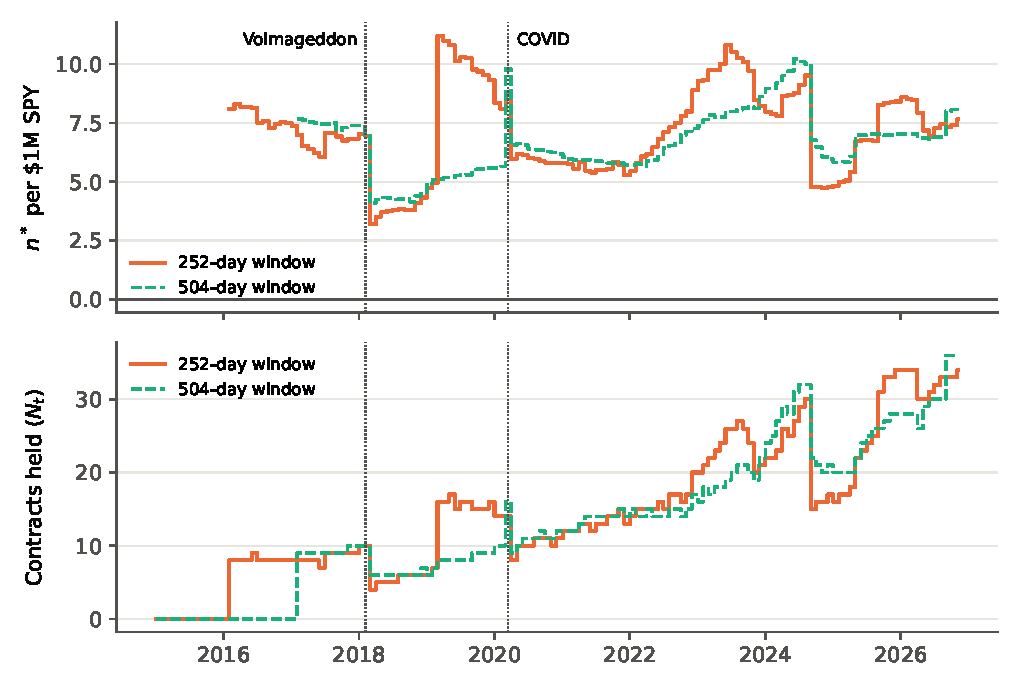
\includegraphics[width=0.95\linewidth]{figures/hedge_ratio_rolling.pdf}
  \caption{Rolling variance-minimizing hedge size. Top: $n^*$ per \$1M of SPY.
  Bottom: actual number of VX contracts held. The first 252 (504) trading days
  are an estimation warm-up with no hedge. Dotted lines mark 5 February 2018
  and 16 March 2020.}
  \label{fig:hedge-ratio}
\end{figure}

\begin{figure}[H]
  \centering
  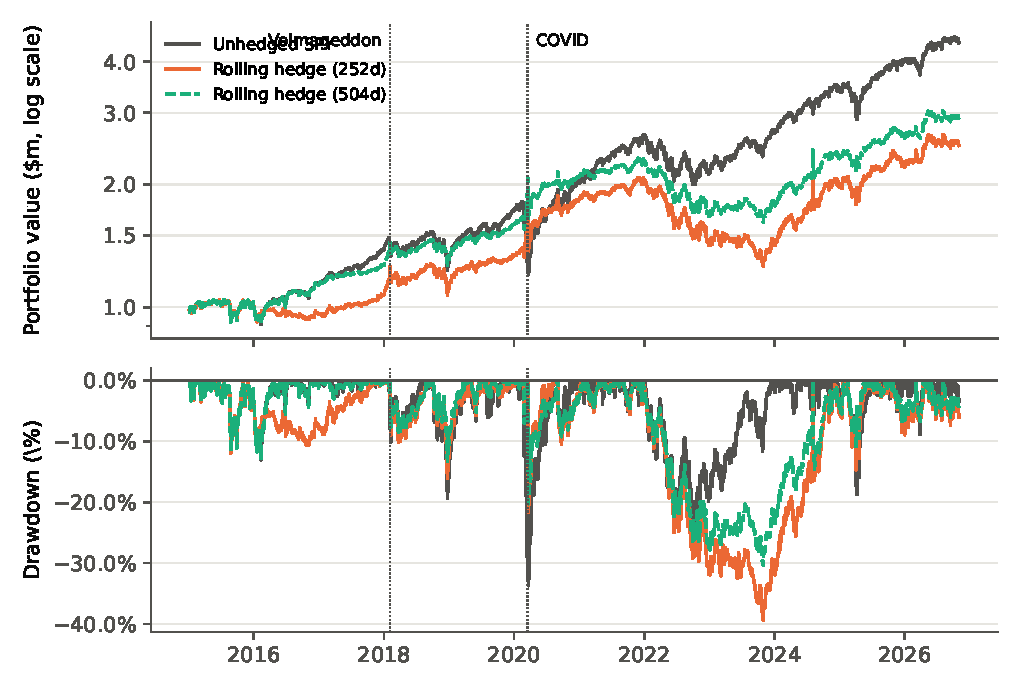
\includegraphics[width=0.95\linewidth]{figures/hedging_equity.pdf}
  \caption{Hedged and unhedged \$1M SPY portfolios. Top: portfolio value on a
  log scale. Bottom: drawdown. The rolling hedge reduces volatility and protects
  in crises, but the 252-day version suffers a prolonged roll-cost drawdown in
  2022--2023.}
  \label{fig:hedging-equity}
\end{figure}

\begin{figure}[H]
  \centering
  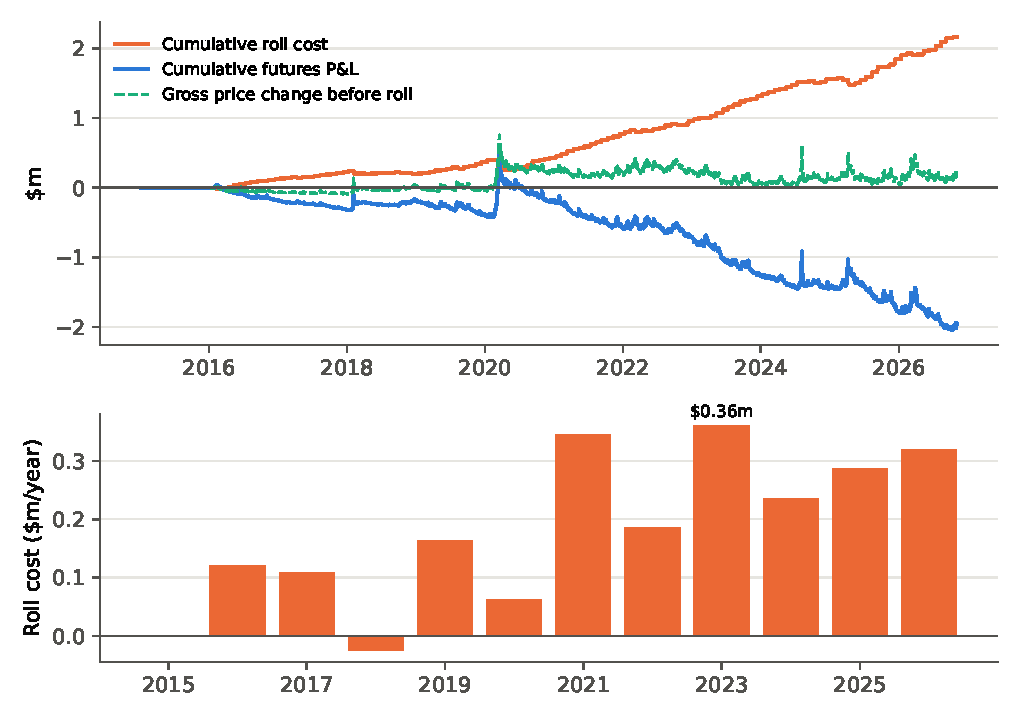
\includegraphics[width=0.95\linewidth]{figures/hedging_roll_cost.pdf}
  \caption{Cumulative roll cost and futures P\&L for the 252-day rolling hedge.
  The roll cost is the dominant drag: gross price change before roll is small.
  Bottom: annual roll cost.}
  \label{fig:hedging-roll-cost}
\end{figure}

\begin{figure}[H]
  \centering
  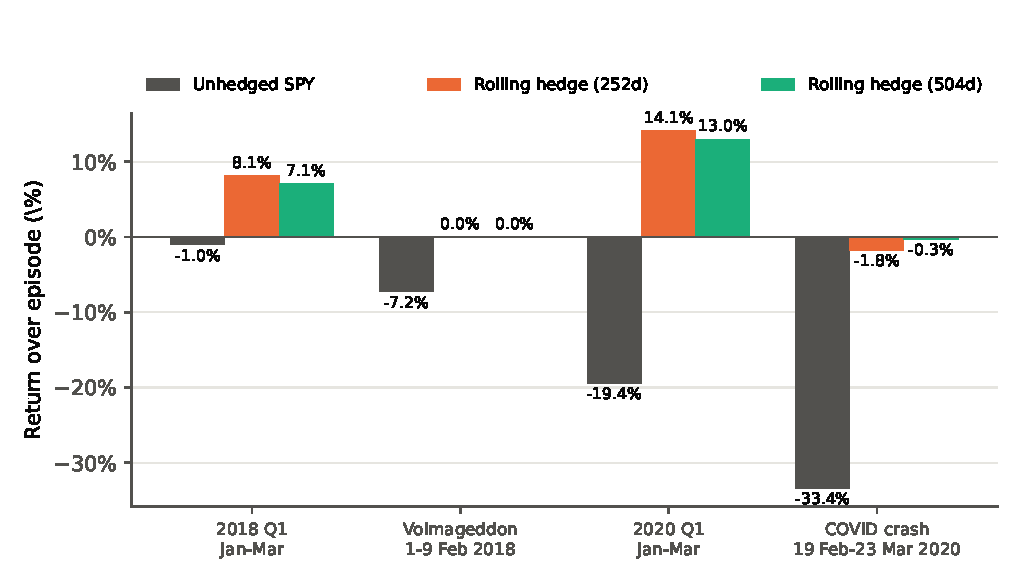
\includegraphics[width=0.95\linewidth]{figures/hedging_crises.pdf}
  \caption{Returns over crisis episodes. The rolling hedge turns the 2020 Q1
  loss into a gain and nearly neutralizes the COVID crash, but over-hedges in
  the calm run-up to 2018.}
  \label{fig:hedging-crises}
\end{figure}
